% Chapter Chapter 11 For Reproducible Research in R and RStudio
% Christopher Gandrud
% Created: 16/07/2012 05:45:03 pm CEST
% Updated: 9 January 2013




\chapter{Presenting with LaTeX}\label{LatexChapter}

By learning how to knit data gathering and analysis LaTeX presentation documents we have already begun to see how LaTeX works for presenting research results. This chapter gives you a more detailed and comprehensive introduction to basic LaTeX document structures and commands. It is not a complete introduction to all that LaTeX is capable of, but we will cover enough that you should be able to create an entire article and slideshow with LaTeX you can use to dynamically present your results. In the next chapter (Chapter \ref{LargeDocs}) we will build on these skills by learning how to use {\emph{knitr}} to create more complex LaTeX documents. 

In this chapter we will learn about basic LaTeX document structures and syntax as well as how to dynamically create LaTeX bibliographies with R and \emph{knitr}. Finally, we will look at how to create PDF slideshow with LaTeX and \emph{knitr}. 

\section{The Basics}

In this section we will look at how to set up a basic LaTeX article including what editors to use, the basic structure of a LaTeX document and LaTeX syntax including how to create footnotes, cross-references, headings, and changing font sizes. I will assume that you already have a fully functioning TeX distribution installed on your computer. See page \pageref{InstallMarkup} for information on how to install TeX.

This book was created using LaTeX. Virtually all tool discussed in this section was used in its creation. Please feel free to look at the markup available on the Book's main GitHub page for examples: \url{}.

\subsection{Getting Started with LaTeX Editors}

As I mentioned earlier, RStudio is a fully functional LaTeX editor as well as an integrated development environment for R. If you want to create a new LaTeX document you can click {\tt{File}} in the menu bar then {\tt{New}} \textrightarrow {\tt{R\; Sweave}}. 

Remember from Chapter \ref{GettingStartedRKnitr} that R Sweave\index{R Sweave} files are basically LaTeX files that can include {\emph{knitr}} code chunks. You can use RStudio to knit and compile a document with the click of one button: \textbf{Compile PDF} (
\includegraphics[scale=0.5]{/git_repositories/Rep-Res-Book/Source/Children/Chapter11/images11/CompilePDF.png}). You can use this button to compile R Sweave files like regular LaTeX files in RStudio even if they do not have code chunks. If you use another program to compile them you might need to change the file extension from {\tt{.Rnw}} to {\tt{.tex}}.

There are many other LaTeX editors\footnote{Wikipedia has collated table comprehensively comparing many of these editors} and many text editors can be modified to compile LaTeX documents. For example, alongside writing this book in RStudio, I typed much of the LaTeX markup in the Sublime Text 2\footnote{http://www.sublimetext.com/} text editor. None of these options have RStudio's high level integration with \emph{knitr}.

\subsection{Basic command syntax}

As you probably noticed in the examples from Part II, LaTeX commands start with the backslash (\texttt{\textbackslash{}}) escape character\index{escape character}. For example, to create a section heading you use the \texttt{section} command. The arguments for LaTeX commands are written inside of curly braces (\verb|{}|) like this:

\begin{knitrout}
    \definecolor{shadecolor}{rgb}{0.969, 0.969, 0.969}
    \color{fgcolor}
    \begin{kframe}
        \begin{verbatim}
\section{My Section Name}
            \end{verbatim}
        \end{kframe}
\end{knitrout}

\noindent Probably one of the biggest sources of compiling errors are caused by curly brackets that aren't closed in that an open bracket (\verb|{|) is not matched by a subsequent closed bracket (\verb|}|). Watch out for this and use an editor (like RStudio) that highlights a brackets matching pair. As we will see, unlike in R with parentheses if your LaTeX command does not have an argument you do not need to include the curly brackets. 

There are a number of helpful lists of LaTeX commands. The Netherlands TeX users group has compiled a comprehensive list. See: \url{http://www.ntg.nl/doc/biemesderfer/ltxcrib.pdf}.

\subsection{The preamble \& the body}\label{LaTeXPreamble}

All LaTeX documents require a preamble\index{LaTeX preamble}. The preamble goes at the very beginning of the document. The preamble usually starts with the \texttt{documentclass}\index{documentclass} command. This specifies what type of presentation document the document is creating--e.g. an article, a book, a slideshow,\footnote{``Slideshow'' is not valid class. One slideshow class that we discuss later is called ``beamer''.} and so on. LaTeX refers to these as classes.\index{LaTeX class} Classes specify a document's formatting. You can add options to \texttt{documentclass} to change the format of the entire document. For example, if we wanted to create an article class document with two columns we would type:

\begin{knitrout}
\definecolor{shadecolor}{rgb}{0.969, 0.969, 0.969}\color{fgcolor}\begin{kframe}
\begin{alltt}
\textbackslash{}documentclass[twocolumn]\{article\}
\end{alltt}
\end{kframe}
\end{knitrout}


In the preamble you can also specify what style it should be formatted in and load any extra packages you may want to use to help you format your document.\footnote{The command to load a package in LaTeX is \texttt{\textbackslash{}usepackage}.\index{usepackage, LaTeX command} For example, if you include \texttt{\textbackslash{}usepackage\{url\}} in the preamble of your document you will be able to specify URL links in the body with the command \texttt{\textbackslash{}url\{SOMEURL\}}.}

The preamble is often followed by the body of your document. It is specified with the \texttt{body} environment.\index{body, LaTeX environment} See Chapter \ref{TablesChapter} page \pageref{LaTeXEnviron} for more details about LaTeX environments. You tell LaTeX where the body\index{LaTeX begin document} of your document starts by typing \verb|\begin{document}|. The very last line of you document is usually \verb|\end{document}|, indicating that your document has ended. When you open a new R Sweave file in RStudio it creates an article class document with a very simple preamble and body like this:

\begin{knitrout}
\definecolor{shadecolor}{rgb}{0.969, 0.969, 0.969}\color{fgcolor}\begin{kframe}
\begin{alltt}
\textbackslash{}documentclass\{article\}

\textbackslash{}begin\{document\}




\textbackslash{}end\{document\}
\end{alltt}
\end{kframe}
\end{knitrout}


\noindent This is all you need to get a very basic article class document working. If you want the document to be of another class simply change \texttt{article} to something else, a \texttt{book} for example.

Let's begin to modify the markup. First we will include in the preamble some the package we need to include clickable hyperlinks (\texttt{hyperref}). Note that in general, and unlike in R, the required packages are already installed on you computer when you installed the TeX distribution.

Next it's often a good idea to include \emph{knitr} code chunks that specify features of the document as a whole. These can include global chunk options\index{global chunk options}, loading data and packages used throughout the document.

Then it's a good idea to specify title information just after the \texttt{document} environment begins. Use the \texttt{title} command to add a title, the \texttt{author} command to add author information and \texttt{data} to specify the date.\footnote{In some document classes the current data will automatically be included if you don't specify the date.} Then include the \texttt{maketitle} command. This will place your title and author information in the body of the document. If you are writing an article you may also want to follow \texttt{maketitle} with an abstract. Unsurprisingly, you can use the \texttt{abstract} environment to include this.

Here is what the document looks like with all of these changes added:

{\scriptsize
\begin{knitrout}
    \definecolor{shadecolor}{rgb}{0.969, 0.969, 0.969}\color{fgcolor}
    \begin{kframe}
        \begin{alltt}
%%%%%%%%%%%%%%  Article Preamble %%%%%%%%%%%%%%
\textbackslash{}documentclass\{article\} 

%% Load LaTeX packages
\textbackslash{}usepackage\{url\}
\textbackslash{}usepackage\{hyperref\}

%% Set knitr global options and gather data
\textless{}\textless{}Global, include=FALSE\textgreater{}\textgreater{}=
\hlcomment{#### Set chunk options ####}
opts_chunk$\hlfunctioncall{set}(fig.align=\hlstring{'center'})

\hlcomment{#### Load and cite R packages ####}
# Create list of packages
PackagesUsed <- c(hl\string{"devtools", "knitr", "ggplot2"})

# Load LoadandCite function
devtools::source_url({hl\string"http://bit.ly/UI95Oq"})

# Load PackagesUsed and creatr .bib BibTeX file
LoadandCite(PackagesUsed, file = \hlstring{"Packages.bib"}, install = FALSE)

\hlcomment{#### Gather Democracy data from Pemstein et al. (2010) ####}
\hlcomment{# For simplicity, store the URL in an object called 'url'.}
url <- \hlstring{"http://bit.ly/S0vxk2"}

\hlcomment{# Create a temporary file called 'temp' to put the zip file into.}
temp <- \hlfunctioncall{tempfile}()

\hlcomment{# Download the compressed file into the temporary file.}
\hlfunctioncall{download.file}(url, temp)

\hlcomment{# Decompress the file and convert it into a dataframe}
\hlcomment{# class object called 'data'.}
UDSData <- \hlfunctioncall{read.csv}(\hlfunctioncall{gzfile}(temp, \hlstring{"uds_summary.csv"}))

\hlcomment{# Delete the temporary file.}
\hlfunctioncall{unlink}(temp)

@

%% Start document body
\textbackslash{}begin\{document\}

%%%%%%%%%%%%% Create title %%%%%%%%%%%%%%%%%
\textbackslash{}title\{An Example knitr LaTeX Article\}
\textbackslash{}author\{Christopher Gandrud \textbackslash{}\textbackslash{}
Hertie School of Governance\textbackslash{}thanks\{Email: \textbackslash{}href\{mailto:gandrud@hertie-school.org\}
\{gandrud@hertie-school.org\}\}\}
\textbackslash{}date\{Janary 2014\}
\textbackslash{}maketitle

%%%%%%%%%%%%% Abstract %%%%%%%%%%%%%%%%%%%%
\textbackslash{}begin\{abstract\}
  Here is an example of a knittable article class LaTeX document.
\textbackslash{}end\{abstract\}

%%%%%%%%%%% Article Main Text %%%%%%%%%%%%%
This article gathers democracy data and graphs it. 

\textbackslash{}section\{The Graph\} 

I gathered data from \textbackslash{}cite\{Pemstein2010\} on countries' democracy level. They call their 
democracy measure the Unified Democracy Score (UDS).

Figure \textbackslash{}ref\{DemPlot\} shows the mean UDS scores over time for all of the countries in their 
sample.

\textbackslash{}begin\{figure\}
    \textbackslash{}caption\{Mean UDS Scores\}
    \textbackslash{}label\{DemPlot\}
\textless{}\textless{}echo=FALSE, message=FALSE\textgreater{}\textgreater{}=
\hlcomment{# Graph UDS scores}
ggplot(UDSData, aes(x = year, y = mean)) +
        stat_smooth() +
        xlab(\hlstring{"Democracy Score"}) + ylab(\hlstring{""}) +
        theme\_bw()
@
\textbackslash{}end\{figure\}

%%%%%%%%%%%%% Reproducing the Document %%%%%%%%%%%%%
\textbackslash{}section*\{Reproducing the Document\}

This document was created using the R version 2.15.2 and the R package \textbackslash{}emph\{knitr\} 
\textbackslash{}citep\{R-knitr\}. It also relied on the R packages \textbackslash{}emph\{devtools\} 
\textbackslash{}citep\{R-devtools\} and \textbackslash{}emph\{ggplot2\} \textbackslash{}citep\{R-ggplot2\}. 
The document can be completely reproduced from source files available on GitHub at: 
\textbackslash{}url\{https://github. com/christophergandrud/Rep-Res-Examples\}.

%%%%%%%%% Bibliography %%%%%%%%%%%%%%%%%%%%
\textbackslash{}\{apa\}
\textbackslash{}\{Main.bib,Packages.bib\}

\textbackslash{}end\{document\}
        \end{alltt}
\end{kframe}
\end{knitrout}
}

\noindent Just few quick notes about some new syntax in this example. First, remember that the percent sign (\%) is LaTeX's comment character. Using it to comment your markup can make it easier to read. Second, as we saw in Chapter \ref{TablesChapter} (page \ref{DoubleBS}) double backslashes (\verb|\\|), like those after the author name, force a new line in LaTeX. We will discuss the \texttt{emph} command in a moment. Third, using the \texttt{thanks}\index{thanks, LaTeX command} allows us to create a footnote for author contact information\footnote{Frequently it also includes thank yous to people who have help the research.} that is not numbered like the other footnotes (see below). Finally, you'll notice \verb|\href{mailto: . . . .org}}|.\index{href, LaTeX command}\index{mailto, LaTeX command} This creates an email address in the final document that will open the reader's default email program when clicked. 

\subsection{Headings}

Now we have set up the beginning of our article. Let's build the body. 
Earlier in the chapter we briefly saw how to create section-level headings with \texttt{section}.\index{section, LaTeX command} There are a number of other sub-section level headings including \texttt{subsection}, \texttt{subsubsection}, \texttt{paragraph}, and \texttt{subparagraph}. Headers are numbered automatically by LaTeX.\footnote{The \texttt{paragraph} level does not have numbers.} To have an unnumbered section place an asterisk in it like this: \verb|\section*{Unnumbered Section}|. In book class documents you can also use \texttt{chapter} to create new chapters and \texttt{part} for collections of chapters.

\subsection{Paragraphs \& spacing}

In LaTeX paragraphs are simply created by adding an blank line between lines. It will format all of the tabs for the beginning of paragraphs based on the document's class rules. As we discussed before, writing tabs in the markup version of your document does nothing in the compiled document. They are generally used just to make the markup easier for people to read. 

Note that adding more blank lines between paragraphs will not add extra space between the paragraphs in the final document. To specify the space following paragraphs (or almost any line) use the \texttt{vspace} (vertical space) command.\index{vspace, LaTeX command} for example to add three centimeters of vertical space on a page type: \verb|\vspace{3cm}|. This gives us the following space:

\vspace{3cm}

Similarly adding extra spaces between words in your LaTeX markup won't create extra spaces between words in the compiled document. To add horizontal space use the \texttt{hspace}\index{hspace, LaTeX command} in the same way as \textt{vspace}.

\subsection{Text formatting \& math}

Let's briefly look at how to do some of the more common types of text formatting in LaTeX and how to create some commonly used diacritics and special characters. We will also briefly look at how to include LaTeX's powerful mathematical typesetting capabilities.

\paragraph{Italics \& Bold}

To italicize a word in LaTeX use the \texttt{emph} (emphasis) command.\index{emph, LaTeX command} For bold use \texttt{textbf}.\index{textbf, LaTeX command} You can nest commands inside of one another to combine their effect. For example, to \emph{\textbf{italicize and bold}} a word use: \verb|\emph{textbf{italicize and bold}}|.

\paragraph{Font size}\label{FontSize}

You can specify the base font size of an entire document with a \texttt{documentclass} option. For example, to create an article with 12 point font use: \texttt{\textbackslash{}documentclass[12pt]\{article\}}.

There are a number of commands to set the size of specific pieces of text relative to the base size. See Table \ref{LaTeXFontSize} for the full list. Usually a slightly different syntax is used for these commands that goes like this: \verb|{\SIZE_COMMAND . . . }|. For example, to use the {\small small size} type: \verb|{\small small size}|.

\begin{table}
    \caption{LaTeX Font Size Commands}
    \label{LaTeXFontSize}
    \begin{center}
        \hline\\[0.25cm]
        \begin{tabular}{c}
            {\Huge \texttt{Huge}} \\
            {\huge \texttt{huge}} \\
            {\LARGE \texttt{LARGE}} \\
            {\Large \texttt{Large}} \\
            {\large \texttt{large}} \\
            {\normalsize \texttt{normalsize}} \\
            {\small \texttt{small}} \\
            {\footnotesize \texttt{footnotesize}} \\
            {\scriptsize \texttt{scriptsize}} \\
            {\tiny \texttt{tiny}} \\[0.25cm]
        \end{tabular}
        \hline
    \end{center}
\end{table}

\noindent You can change the size of code chunks that \emph{knitr} places in presentation documents using these commands. Just place the code chunk inside of \verb|{\SIZE_COMMAND . . . }|.

\paragraph{Diacritics}\index{diacritics, LaTeX}

You cannot directly enter letters with diacritics--e.g. accent mark--into LaTeX directly. For example to create a letter c with a cedilla (\{c}) you need to type \verb|\{c}|. To create an `a' with an acute accent (\'{a}) type: \verb|\'{a}|. There are obviously many types of diacritics and commands to include them in LaTeX produced documents. For a comprehensive discussion of the issue and a list of commands see the LaTeX Wikibook page on the topic: \url{http://en.wikibooks.org/wiki/LaTeX/Special_Characters}. If you regularly use non-English alphabets you might also be interested in reading the LaTeX Wikibook page on on internationalization: \url{http://en.wikibooks.org/wiki/LaTeX/Internationalization}.

\paragraph{Quotation marks}

To specify double left quotation marks (``) use two back ticks (\verb|``|). For double right quotes use the usual double quote character ("). Single quotes follow the same format (\verb|`'|). 

\paragraph{Math}\index{math, LaTeX}

LaTeX is particularly popular among quantitative researchers and mathematicians because is very good at rendering mathematics. A complete listing of every math command would take up quite a bit of space.\footnote{See the Netherlands TeX user group list mentioned earlier for an extensive compilation of LaTeX math commands.} I am briefly just going to discuss how to include math in a LaTeX document. This discussion includes a few math examples. 

To include math inline with your text place the math in between two dollar signs (\verb|$$|). For example, \verb|$s^{2} = \frac{\sum(x - \bar{x}^2)}{n - 1}$| produces $s^{2} = \frac{\sum(x - \bar{x}^2)}{n - 1}$ in our final document.\footnote{Instead of dollar signs you can also use \textbackslash{}( . . . \textbackslash).} We can display math separate from the text with two dollar signs on either side of our math commands (\verb|$$ . . . $$|).\footnote{Equivalently, use \textbackslash{}[ . . . \textbackslash{}] or the \texttt{display} environment. To number display equations use the \texttt{equation} environment.} For example, 

\begin{knitrout}
\definecolor{shadecolor}{rgb}{0.969, 0.969, 0.969}\color{fgcolor}\begin{kframe}
\begin{verbatim}
$$
s^{2} = \frac{\sum(x - \bar{x}^2)}{n - 1}
$$
\end{verbatim}
\end{kframe}
\end{knitrout}


\noindent gives us:

$$
s^{2} = \frac{\sum(x - \bar{x}^2)}{n - 1}
$$

\subsection{Lists}\index{LaTeX lists}

To create lists in LaTeX use the \texttt{itemize}\index{itemize, LaTeX environment} environment. Each list item is delimited with the \texttt{item}\index{item, LaTeX command} command. For example:

\begin{knitrout}
\definecolor{shadecolor}{rgb}{0.969, 0.969, 0.969}\color{fgcolor}\begin{kframe}
\begin{alltt}
\textbackslash{}begin\{itemize\}
    \textbackslash{}item The first item.
    \textbackslash{}item The second item.
    \textbackslash{}item The third item.
\textbackslash{}end\{itemize\}
\end{alltt}
\end{kframe}
\end{knitrout}


\noindent gives us:

\begin{itemize}
    \item The first item.
    \item The second item.
    \item The third item.
\end{itemize}

\noindent To create a numbered list use the \texttt{enumerate}\index{enumerate, LaTeX environment} environment instead of \texttt{itemize}. You can create sublists simply by nesting lists inside of lists like this: 

\begin{knitrout}
\definecolor{shadecolor}{rgb}{0.969, 0.969, 0.969}\color{fgcolor}\begin{kframe}
\begin{alltt}
\textbackslash{}begin\{itemize\}
    \textbackslash{}item The first item.
    \textbackslash{}item The second item.
    \textbackslash{}begin\{itemize\}
        \textbackslash{}item A sublist item
    \textbackslash{}end\{itemize\}
    \textbackslash{}item The third item.
\textbackslash{}end\{itemize\}
\end{alltt}
\end{kframe}
\end{knitrout}


\noindent which gives us:

\begin{itemize}
    \item The first item.
    \item The second item.
    \begin{itemize}
        \item A sublist item
    \end{itemize}
    \item The third item.
\end{itemize}

\subsection{Footnotes}

Plain, non-bibliographic footnotes are easy to create in LaTeX. Simply place \texttt{\textbackslash{}footnote\{} where you would like the footnote number to appear in the text. Then type the footnote's text. Of course remember to close the footnote with a \texttt{\}}. LaTeX does the rest, including formatting and numbering.

\subsection{Cross-References}

LaTeX will also automatically format cross-references. We were already partially introduced to cross-references in chapters \ref{TablesChapter} and \ref{FiguresChapter}. At the place where you would like to refer to add a \texttt{label} such as \verb|\label{ACrossRefLabel}|.\index{label, LaTeX command} It doesn't really matter what label you choose, though make sure they are not duplicated in the document. Also, it can be a good idea to use the same conventions that we learned for labeling R objects (see page \pageref{ObjectNames}). Then place a \texttt{ref}\index{ref. LaTeX command} command (e.g. \verb|\ref{ACrossRefLabel|) at the place in the text where you want the cross-reference to be. 

If you place the \texttt{label} on the same line as a heading command \texttt{ref} will place the heading number. If \texttt{label} is in a \texttt{table} or \texttt{figure} environment you will get the table or figure number. You can also use \texttt{pageref} instead of \texttt{ref} to include the page number. Finally, loading the \emph{hyperref} package makes cross-references (or footnote) clickable. Clicking on them will take you to the item the reference is referring to.

\section{Bibliographies with BibTeX}\label{BibTeXBib}\index{BibTeX}\index{bibliographies, LaTeX}

LaTeX can take advantage of very comprehensive bibliography making capabilities. All major TeX distributions come with BibTeX. BibTeX is basically a tool for creating databases of citation information. In this section, we are going to see how to incorporate a BibTeX bibliography into you LaTeX documents. Then we will learn how use R to automatically generate a bibliography of packages used to create a knitted document. We will cover very basic BibTeX syntax. For more information see the LaTeX Wikibook page on Bibliography management: \url{http://en.wikibooks.org/wiki/LaTeX/Bibliography_Management}.

\subsection{The \emph{.bib} file}

BibTeX bibliographies are stored in plain-text files with the extension \emph{.bib}. These files are databases of citations.\footnote{The order of the citations does not matter.} The syntax for each citation goes like this:

\begin{knitrout}
    \definecolor{shadecolor}{rgb}{0.969, 0.969, 0.969}\color{fgcolor}
    \begin{kframe}
        \begin{alltt}
@DOCUMENT_TYPE\{CITE_KEY,
    title = \{TITLE\},
    author = \{AUTHOR\},
    . . . = \{. . .\}
\} 
        \end{alltt}
\end{kframe}
\end{knitrout}

\noindnet \verb|DOCUMENT_TYPE| specifies what type of document--article, book, webpage, and so on--the citation is for. This determines what items the citation can and needs to include. Then we have the \verb|CITE_KEY|.\index{BibTeX citation keys} This is the reference's label that you will use to include the citation in your presentation document. We'll look more at this later in the section. Each citation must have a unique \verb|CITE_KEY|. A common way to write these keys is to use the author's surname and the publication year, e.g. \verb|Donohue2009|. The cite key is followed by the other citation attributes such as \texttt{author}, \texttt{title} and \texttt{year}. These attributes all follow the same syntax: \verb|ATTRIBUTE = {. . .}|.

It's worth taking a moment to discuss the syntax for the BibTeX author attribute. First multiple author names are separated by \texttt{and}. Secondly, BibTeX assumes that the last word for each author is their surname. If you would like multiple words to be taken as the ``surname'' then enclose these word's in curly brackets. If we wanted to cite the World Bank as an author we write \verb|{World Bank}|, otherwise it will be formatted Bank, World in the presentation document.

Here is a complete BibTeX entry for \cite{Donohue2009}:

\begin{knitrout}
    \definecolor{shadecolor}{rgb}{0.969, 0.969, 0.969}\color{fgcolor}
    \begin{kframe}
        \begin{alltt}
@article\{Donohue2009,
  author = \{David L Donohue and Arian Maleki and Morteza 
  Shahram and Inam Ur Rahman and Victoria Stodden\},
  title = \{Reproducible Research in Computational Harmonic 
  Analysis\},
  journal = \{Computing in Science \& Engineering\},
  year = \{2009\},
  volume = \{11\},
  number = \{1\},
  pages = \{8--18\}
\}
        \end{alltt}
\end{kframe}
\end{knitrout}

\noindent Each item of the entry must end in a comma, except the last one.\footnote{This is very similar to how we create vectors in R.} 

\subsection{Including citations in a LaTeX document}

When you want to include citations from a BibTeX file in your LaTeX document you first use the \texttt{bibliography}\index{bibliography, LaTeX command} command. For example, if the BibTeX file is called \emph{Main.bib} and it is in the same directory as your markup document then type: \verb|\bibliography{Main.bib}|. You can used a bibliography stored in another directory, just include the appropriate file path information. Usually \texttt{bibliography} is placed right before \verb|\end{document}| so that it appears at the end of the compiled presentation document.

You can also specify how you would like the references to be formatted using the \texttt{bibliographystyle}\index{bibliographystyle} command. For example, this book uses the American Psychological Association (APA) style for references. To set this I included \verb|\bibliographystyle{apa}| directly before \texttt{bibliography}. The default style\footnote{It is referred to in LaTeX as the plain style.} is to number citations (e.g. [1]) rather than the author-year style\footnote{This is sometimes referred to as the ``Harvard'' style.} used by the APA. You will need to include the LaTeX package \emph{natbib}\index{Natbib} to be able to use author-year citation styles. This book includes \verb|\usepackage[authoryear]{natbib}| in it's preamble.

Place the \texttt{cite}\index{cite, LaTeX command} command in your document's text where you want to place a reference. You include the \verb|CITE_KEY| for the reference in this command, e.g. \verb|\cite{Donohue2009}|. You can include multiple citations in \texttt{cite}, just separate the \verb|CITE_KEY|s with commas. You can add options such as the page numbers of other text to a citation using square brackets ([]). For example if we wanted to cite the tenth page of \cite{Donohue2009} we type: \verb|\cite[10]{Donohue2009}|. The author-year style in-text citation this produces looks like this: \cite[10]{Donohue2009}. You can add text at the beginning of a citation with another set of square brackets. Typing \verb|\cite[see][10]{Donohue2009}| gives us \cite[see][10]{Donohue2009}.

If you are using an author-year style you can use a variety of \emph{natbib} of commands to change how what information is included in the parentheses. For a selection of these commands and examples see Table \ref{NatbibTable}.

\begin{table}
    \caption{A Selection of \emph{natbib} In-text Citation Style Commands}
    \label{NatbibTable}
        \begin{center}
            \begin{tabular}{l r}
                \hline
                Command Example & Output \\[0.25cm]
                \hline\hline
                \verb|\cite{Donohue2009}| & \cite{Donohue2009} \\
                \verb|\citep{Donohue2009}| & \citep{Donohue2009} \\
                \verb|\citeauthor{Donohue2009}| & \citeauthor{Donohue2009} \\
                \verb|\citeyear{Donohue2009}| & \citeyear{Donohue2009} \\
                \verb|\citeyearpar{Donohue2009}| & \citeyearpar{Donohue2009} \\
                \hline
            \end{tabular}
        \end{center}
\end{table}

\subsection{Generating a BibTeX file of R packages}

Researchers are pretty good about consistently citing others' articles and data. However, citations of R packages used in analyses is very inconsistent. This is unfortunate not only because correct attribution is not being given to those who worked to create the package, but also because it makes reproducibility harder. It obscures important steps that were taken in the research process, primarily which package versions were used. Fortunately, there are R tools for quickly and dynamically generating citations, including the versions of the packages you are using. It can also add them directly to an existing bibliography file.

You can automatically create citations for R packages using the \texttt{citation}\index{citation, R command} command inside of a code chunk. For example if you want the citation information for the \texttt{xtable} package you would simply type:

{\small
\begin{knitrout}
\definecolor{shadecolor}{rgb}{0.969, 0.969, 0.969}\color{fgcolor}\begin{kframe}
\begin{alltt}
\hlfunctioncall{citation}(\hlstring{"xtable"})
\end{alltt}
\begin{verbatim}
## 
## To cite package 'xtable' in publications use:
## 
##   David B. Dahl (2012). xtable: Export tables to LaTeX or HTML. R
##   package version 1.7-0. http://CRAN.R-project.org/package=xtable
## 
## A BibTeX entry for LaTeX users is
## 
##   @Manual{,
##     title = {xtable: Export tables to LaTeX or HTML},
##     author = {David B. Dahl},
##     year = {2012},
##     note = {R package version 1.7-0},
##     url = {http://CRAN.R-project.org/package=xtable},
##   }
## 
## ATTENTION: This citation information has been auto-generated from
## the package DESCRIPTION file and may need manual editing, see
## 'help("citation")' .
\end{verbatim}
\end{kframe}
\end{knitrout}

}

\noindent This gives you both the plain citation as well as the BibTeX version. If you only want the BibTeX version of the citation you can use the \texttt{toBibtex} command.\index{toBibTeX}

\begin{knitrout}
\definecolor{shadecolor}{rgb}{0.969, 0.969, 0.969}\color{fgcolor}\begin{kframe}
\begin{alltt}
\hlfunctioncall{toBibtex}(\hlfunctioncall{citation}(\hlstring{"xtable"}))
\end{alltt}
\begin{verbatim}
## @Manual{,
##   title = {xtable: Export tables to LaTeX or HTML},
##   author = {David B. Dahl},
##   year = {2012},
##   note = {R package version 1.7-0},
##   url = {http://CRAN.R-project.org/package=xtable},
## }
\end{verbatim}
\end{kframe}
\end{knitrout}


The {\emph{knitr}} package create BibTeX bibliographies for R packages with the \texttt{write\_bib}\index{write\_bib} command. Let's make a BibTeX file called \emph{Packages.bib} containing citation information for the \emph{xtable} package.

\begin{knitrout}
\definecolor{shadecolor}{rgb}{0.969, 0.969, 0.969}\color{fgcolor}\begin{kframe}
\begin{alltt}
\hlcomment{# Create package BibTeX file}
knitr::\hlfunctioncall{write_bib}(\hlstring{"xtable"},
                 file = \hlstring{"Packages.bib"})
\end{alltt}
\end{kframe}
\end{knitrout}


\noindent \verb|write_bib| automatically assigns each entry a cite key using the format \verb|R-PACKAGE_NAME|, e.g. \verb|R-xtable|.

\textbf{Warning:} The \emph{knitr}'s \verb|write_bib| command currently does not have the ability to append the citations to an existing file, but instead writes them to a new file. If there is already a file with the same name it will overwrite the file. So, be very careful using this command to avoid accidental deletions. Therefore it is good to have \verb|write_bib| always write to a file specifically for automatically generated package citations. You can include more than one bibliography in LaTeX's \texttt{bibliography} command. All you need to do is separate them with a comma.

\begin{knitrout}
\definecolor{shadecolor}{rgb}{0.969, 0.969, 0.969}\color{fgcolor}\begin{kframe}
\begin{alltt}
\textbackslash{}bibliography\{Main.bib,Packages.bib\}
\end{alltt}
\end{kframe}
\end{knitrout}


We can use these techniques to automatically create a BibTeX file with citation information for all of the packages used in a research project. Simply make a character vector of the names of package that you would like to include in your bibliography. Then run this through \verb|\write_bib|. 

You can make sure you are citing all of the key packages used in a knitted document by (a) creating a vector of all of the packages and then (b) using this to both load the packages and write the bibliography. Here is an example:

\begin{knitrout}
\definecolor{shadecolor}{rgb}{0.969, 0.969, 0.969}\color{fgcolor}\begin{kframe}
\begin{alltt}
\hlcomment{# Package list}
PackagesUsed <- \hlfunctioncall{c}(\hlstring{"ggplot2"}, \hlstring{"knitr"}, \hlstring{"xtable"}, \hlstring{"Zelig"})

\hlcomment{# Load packages}
\hlfunctioncall{lapply}(PackagesUsed, library, character.only = TRUE)

\hlcomment{# Create package BibTeX file}
knitr::\hlfunctioncall{write_bib}(PackagesUsed, file = \hlstring{"Packages.bib"})
\end{alltt}
\end{kframe}
\end{knitrout}


\noindent In the first executable line we just create our list of packages to load and cite. The next command is \texttt{lapply}\index{lapply} (list apply). This applies the function \texttt{library} to all of the items in \emph{PackagesUsed}. \texttt{character.only = TRUE} is a \texttt{library} argument that allows us to use character string versions of the library names as R sees them in the \emph{PackagesUsed} vector, rather than as objects (how we have used library up until now).

If you include these commands in a code chunk at the beginning of your knitted document then you can be sure that you will have a BibTeX file with all of the packages you use.\footnote{I have created a simple function combining these steps as well as the ability to install the listed packages. It is on the Book's GitHub Example repository and can be downloaded into R like this: \texttt{devtools::source\_url("http://bit.ly/UI95Oq")}.}

\section{Presentations with LaTeX Beamer}

You can make slideshow presentations with a number of LaTeX document classes. Creating a presentation with a markup language can take a bit more effort than using a WYSIWYG program like Microsoft PowerPoint\index{Microsoft PowerPoint} or Apple's Keynote.\index{Apple Keynote} However, combining LaTeX and \emph{knitr} can create slideshows fully reproducible presentations that dynamically create and present results. I have found this particularly useful in my teaching as dynamically produced presentations allow me to provide my students with fully replicable examples of how I created a figure on a slide, for example. \emph{knitr} also makes it easy to beautifully present code examples.

One of the most popular is the Beamer class.\index{Beamer} When you compile a Beamer class document a PDF will be created where every page is a different slide (see Figure \ref{BeamerExample}). All major PDF viewer programs have some sort of ``View Full Screen'' option to view Beamer PDFs as full screen slideshows. Usually you can navigate through the slides with the forward and back arrows on the keyboard.

In this section we will take a brief look at the basics of creating slideshows with Beamer, highlighting special considerations that need to be made when working with Beamer and \emph{knitr}. A full example of a knittable Beamer presentation with illustrations of the many of the points discussed here is printed at the end of the chapter.

\begin{figure}
    \caption{Knitted Beamer PDF Example}
    \label{BeamerExample}
        \begin{center}
            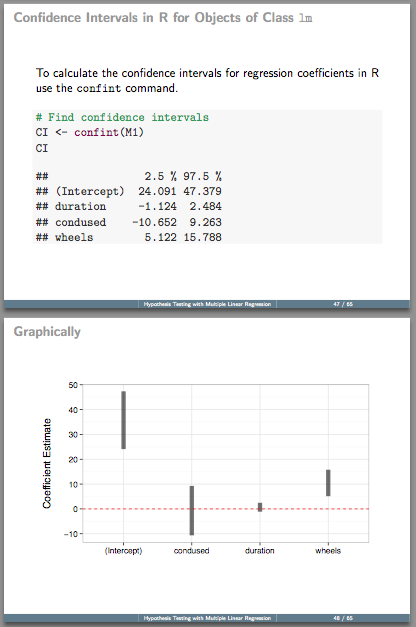
\includegraphics[scale=0.5]{/git_repositories/Rep-Res-Book/Source/Children/Chapter11/images11/BeamerExample.png}
        \end{center}
        {\scriptsize The presentation in this example was created using a custom Beamer theme available at: \url{https://github.com/christophergandrud/Make-Projects/tree/master/Rnw_Lecture}.}
\end{figure}

\subsection{Beamer basics}

{\emph{Knitr}} largely works the same way in in LaTeX slideshows as it does in article or book class documents. There are a few differences to look out for. 

\paragraph{The Beamer preamble}

You use \texttt{documentclass} to set a LaTeX document as a \texttt{beamer} slideshow. You can also include global style information in the preamble by using the commands \texttt{usetheme}, \texttt{usecolortheme}, \texttt{useinnertheme}, \texttt{useoutertheme}. For a fairly comprehensive compilation of Beamer themes see the Hartwork's Beamer theme matrix: \url{http://www.hartwork.org/beamer-theme-matrix/}. 

\paragraph{Slide frames}

After the preamble you start your document as usual by beginning the \texttt{document} environment. Then you need to start creating slides. Individual beamer slides are created using the \texttt{frame}\index{frame, LaTeX command} environments. Create a frame title using \texttt{frametitle}.\index{frametitle, LaTeX command}

\begin{knitrout}
    \definecolor{shadecolor}{rgb}{0.969, 0.969, 0.969}
    \color{fgcolor}
    \begin{kframe}
        \begin{verbatim}
\frame{
        \frametitle{An example frame.}


}
        \end{verbatim}
    \end{kframe}
\end{knitrout}

\noindent Note that you can also use the usual \verb|\begin{frame} . . \end{frame}| syntax.

Unlike in a WYSIWYG slide show program, you will not be able to tell if you have tried to more information on one slide until after you compile the document.\footnote{One way to deal with frames that go over multiple slides is to use the \texttt{allowframebreaks} command, i.e. \texttt{\textbackslash{}begin\{frame\}[allowframebreaks].\index{allowframebreaks, LaTeX command}.}

\paragraph{Title frames}

One important difference from regular a LaTeX article is that dinstead of using \texttt{maketitle} to place your title information, in Beamer you place the \texttt{titlepage}\index{titlepage, LaTeX command} inside of a frame by itself. 

\paragraph{Sections \& Outlines}

We can use \texttt{section} commands in much the same way as we do in other types of LaTeX documents. Section commands do not need to be placed inside of frames. After the title slide, many slideshows have a presentation outline. You can automatically create one of from your section headings using the \texttt{tableofcontents}\index{tableofcontents, LaTeX command} command. Like the \texttt{titlepage} command, \texttt{tableofcontents} can go on its own frame, i.e.

<<Ch11ToCTitle, eval=FALSE>>
%%% Title slide
\frame{
    \titlepage
}

%% Table of contents slide
\frame{
    \frametitle{Outline}
        \tableofcontents
}
@

\paragraph{Make list items appear}

Lists work the same way in Beamer as they do in other LaTeX document classes. They do have an added feature in that you can have each item appear as you progress through the slide show. After \verb|\item| place the number of the order in which the item should appear. Enclose the number in \verb|< ->|. For example, 

\begin{knitrout}
\definecolor{shadecolor}{rgb}{0.969, 0.969, 0.969}\color{fgcolor}\begin{kframe}
\begin{alltt}
\textbackslash{}begin\{itemize\}
    \textbackslash{}item<1-> The first item.
    \textbackslash{}item<2-> The second item.
    \textbackslash{}item<2-> The third item.
\textbackslash{}end\{itemize\}
\end{alltt}
\end{kframe}
\end{knitrout}


\noindent In this example the first item will appear before the next two. These two will appear at the same time.

\subsection{knitr with LaTeX slideshows}

\noindent \emph{knitr} code chunks have the same syntax in LaTeX slideshows as in other LaTeX documents. You do need to make one change to the \texttt{frame} options however to include highlighted {\emph{knitr}} code chunks on your slides. You should add the \texttt{fragile} option to the \texttt{frame} command.\footnote{For a detailed discussion of why you need to use the \texttt{fragile} option with the verbatim environment that {\emph{knitr}} uses to display highlighted text in LaTeX documents see this blog post by Pieter Belmans: \url{http://pbelmans.wordpress.com/2011/02/20/why-latex-beamer-needs-fragile-when-using-verbatim/} (posted 20 February 2011).} Here is an example:

\begin{knitrout}
    \definecolor{shadecolor}{rgb}{0.969, 0.969, 0.969}
    \color{fgcolor}
    \begin{kframe}
        \begin{verbatim}
\begin{frame}[fragile]
    \frametitle{An example fragile frame.}

\end{frame}
            \end{verbatim}
        \end{kframe}
\end{knitrout}

\noindent Here is a complete knittable Beamer example:

{\scriptsize
\begin{knitrout}
    \definecolor{shadecolor}{rgb}{0.969, 0.969, 0.969}\color{fgcolor}
    \begin{kframe}
        \begin{alltt}
\documentclass\{beamer\}

\begin\{document\}

%% Title page inforamtion
\textbackslash{}title\{Example Beamer/\textbackslash{}emph\{knitr\} Slideshow\}
\textbackslash{}author\{\textbackslash{}href\{mailto:gandrud@yonsei.ac.kr\}\{Christopher Gandrud\}\}

%%% Title slide
\textbackslash{}frame\{
    \textbackslash{}titlepage
\}

%% Table of contents slide
\textbackslash{}frame\{
    \textbackslash{}frametitle\{Outline\}
    \textbackslash{}tableofcontents
\}

%%% The code
\textbackslash{}section\{Access the code\}
\textbackslash{}begin\{frame\}[fragile]
    \textbackslash{}frametitle\{Access the code\}
        The code to create the following figure is available online.
    
        To access it we can type:
\begin{knitrout}
\definecolor{shadecolor}{rgb}{0.969, 0.969, 0.969}\color{fgcolor}\begin{kframe}
\begin{alltt}
\textbackslash{}hlcomment\{\hlcomment{# Access and run the code to create a caterpillar plot\}}
devtools::source\textbackslash{}\hlfunctioncall{_url}(\textbackslash{}hlcomment\{\hlstring{"http://bit.ly/VRKphr"}\})
\end{alltt}
\end{kframe}
\end{knitrout}

\textbackslash{}end\{frame\}

%%% The figure
\textbackslash{}section\{The Figure\}
\textbackslash{}begin\{frame\}[fragile]
    \textbackslash{}frametitle\{The resulting figure\}


